\documentclass[UTF8]{ctexart}

\usepackage{amsmath}
%\usepackage{IEEEtran}
\usepackage[a4paper,left=3cm,right=3cm,top=3cm,bottom=3cm]{geometry} %定制页面和边距
\pagestyle{plain}  %定制页面编号的位置
\usepackage{listings}   %定制代码环境
\lstset{flexiblecolumns}
\usepackage{booktabs}  %定制表格环境
\usepackage{makecell}
\usepackage{float}   %定制浮动的环境
\usepackage{graphicx}
\usepackage{titlesec}    %定制paragraph的转行
\usepackage{tabularx}
\usepackage{longtable}   %用于长表格
\usepackage{array}
\usepackage{subfigure}
\usepackage{cite}
\usepackage{hyperref}
\usepackage{url}
\usepackage{dcolumn}
\usepackage{xtab}

\title{模型检验}
\author{王逸轩 \and 韩啸}
\date{\today}
\CTEXsetup[name={,}]{part} %定制part名
\renewcommand{\abstractname}{\large 摘\ 要}    %定制摘要的名字
\renewcommand\theequation{\thesection.\arabic{equation}}   %定制方程编号
\titleformat{\paragraph}[block]{\normalsize\bfseries}{\theparagraph}{1em}{}   %定制paragraph的转行
\bibliographystyle{unsrt}   %定制文献样式

\linespread{1.6}
\begin{document}
\zihao{-4}
\maketitle






\section{问题的分析}
利用题中所给的条件以及需解决的问题,进行如下分析。

题目要求完成一个模型检验的程序,使得我们可以根据输入的迁移状态系统$TS$和逻辑公式$L$(其中公式可能具有多种类型,如线性时序逻辑公式$LTL$、$CTL$、$CTL$*、$PCTL$、$TCTL$),判断逻辑公式是否得到满足,并在不满足的情况下输出反例。

我们构建的模型需要解决以下的数据结构与算法的核心问题:

(1)将迁移状态系统$TS$给定量刻画下来,方便构造算法进行检验。

(2)刻画逻辑公式$L$,并建立对于公式的一些运算法则(如取子式、递推等等),进一步针对公式进行判断。

(3)针对不同的公式类型,设计算法。

\section{问题的假设与简化}
针对模型的实现,我们做出以下合理且不失一般性的简化:

(1)假设初始输入的逻辑公式,已经指明了公式类型,并且按照运算次序添入了相应的括号。(即公式内部任两个算符合成之后都会添加括号)

(2)为了简化起见,我们这里只对于$LTL$、$CTL$两种情况进行了处理,但从设计的算法容易看出,$CTL$采用的逆推算法也可以援引到解决$CTL$*、$PCTL$、$TCTL$的问题上来。

(3)对于$CTL$的算法,我们没有设计给出反例这一环节,这是由于对于逻辑公式$L$,它本身不成立的反例,就等价于它的否命题成立的实例,而它的否命题本身也构成一个$CTL$逻辑公式,但我们知道,说明一个$CTL$逻辑公式成立可能需要给出无穷多个例子,于是举反例本身便失去了意义。另外,举反例的过程,本质上就是把$CTL$逻辑公式检验的过程重复了一遍,并不能从单一的例子直接观察出$CTL$逻辑公式不成立,于是我们便略去这一环节。

\section{具体模型的设计}
针对问题分析中的几个问题,我们做出如下的模型设计:

首先,我们利用一个图结构储存迁移状态系统$TS$,特别地,我们的数据结构是基于图的邻接表表示。然后我们利用字符串存储逻辑公式,并根据其类型做下一步判断。

接下来,对于$CTL$逻辑公式,我们采用逆推算法,本质上的思想是找到每个逻辑公式对应的满足该公式的节点集合。这样一来,我们在解决了最简单的公式对应的节点集合之后,就可以对于复杂的公式,利用逆推算法,脱去最外层的括号,找到相应的节点集合。最后通过原始逻辑公式$L$找到的相应节点集合,判断迁移状态系统$TS$的初始节点是否在该集合中即可。

对于$LTL$逻辑公式,情况则需要相对更加复杂一些,我们注意到简单的逆推并不一定会带来公式长度的减少,于是逆推过程可能会无限持续下去!这时我们注意到{\emph{Principles of Model Checking}}这本书中关于有限状态机的描述,结合\href{https://moves.rwth-aachen.de/teaching/ss-16/ss16introduction-to-model-checking/}{\emph{Introduction to Model Checking}}这门课程的PPT资源中一些详尽的具体事例说明,我们引入这种思想设计模型,取得了出人意料的成效:检验与反例枚举这两个步骤在这种观点下都变得迎刃而解了,我们只需经过一次判断就可以一举完成这两项目标。

最后,我们整合前述的分析,设计模型,调整输入和输出即可。

\section{实现中的关键问题和技术分析}
正如在模型设计这一部分所提到的,我们实现模型的关键问题是解决$CTL$逻辑公式中的逆推算法,以及利用有限状态机处理$LTL$逻辑公式。此外,我们需要选取恰当的方法来处理输入输出的问题。

\subsection{逆推算法的设计}
这一部分主要通过讨论最外层运算符来完成,当最外层不为${\forall}$、${\exists}$这两个算符时,我们利用朴素的递归就能快速逆推;否则我们借用$callastE$、$callastA$这两个递归函数来处理。

\subsection{有限状态机思想的处理}
这个环节是整个程序最复杂、也最难理解的部分。注意到前面提到的逆推算法可能会让公式变长,我们需要简化公式,减少那些需要无穷多次判断的算符的数量和类别,即第一步基本的操作是我们首先把输入的$LTL$逻辑公式$S$进行简化,用$U$“直到”算符来表示$W$“弱直到”、$D$“最终满足”、$S$“一直满足”等算符。接下来,我们把逻辑公式$S$的所有子串给记录下来,然后这些子串形成一个集合(为了简化计算复杂度的考虑,我们只需考察最外层没有否定符号$!$的子串),我们考察这个集合生成的子集族$Q$,子集族中每个元素代表着相应的子串得到了满足,而余下的子串没有得到满足,对于$Q$中的每个元素,它应该是某个路径确实满足的子串构成的集合,于是我们进行一步筛查筛掉不合理的元素。我们考察一个新的图$G_{1}$,节点集合是由原来的节点集合$V$与新得到的子集族$Q$形成的的笛卡尔积,我们设法把原来的迁移状态系统$TS$存在反例的问题转化为新图$G_{1}$存在一条满足某种性质的路径的问题,这样一来通过对$G_{1}$的深度搜索即可完成结论。

具体来说,新的图$G_{1}$中的二元对顶点$(v, q)$,其中$v\in V$、$q\in Q$,这个顶点的含义是原来图$G$中的顶点$v$的某条路径满足的子串集合,恰好构成$q$。于是存在一条反例的路径,就要求有一条路径,初始点为迁移状态系统$TS$的起始节点$v_{0}$,初始满足的子串集合在子集族$Q_{0}$中,其中$Q_{0}$是所有表示$S$没有得到满足的的元素$q\in Q$构成的集合。这条路径循环下去,我们把每个节点依次对应到$G_{1}$中的一个节点,就得到了$G_{1}$中的一个无穷长路径。这个无穷长路径我们可以通过对于图$G_{1}$的深度搜索来得到,但为了简化运算量,我们先进行一步筛查来判断哪些图$G_{1}$中的点连有边,即原图$G$中哪些状态可以相互转化。这样的等价刻画给出之后,最后利用下面所示的关键定理,处理我们需要无穷次判断的$U$“直到”算符。即我们知道,存在的反例即需要把每个$U$“直到”算符满足无穷次,我们找到反例路径里重复出现无穷次的点$(v, q)$,于是对于每个$U$“直到”算符,存在某条经过$(v, q)$的闭合回路,其中某个点满足这个算符。于是最终我们一举得到是否存在反例,并给出具体的例子,其中具体的例子是用回路给出,本质上是把所有$U$“直到”算符的例子的环路路径拼接到一起,我们通过前面的定理不难论证,所有的反例都可以转化为回路形式给出,并且给出的路径的确构成一个反例。

\begin{figure}[htbp]
\centering
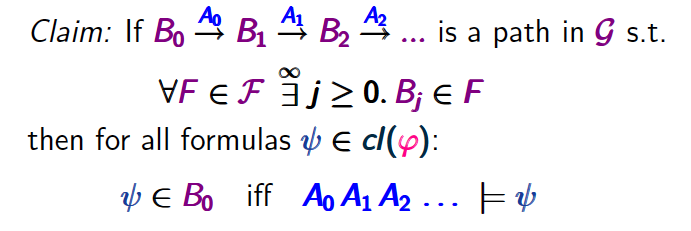
\includegraphics[scale=0.5]{Figure_1.png}
\end{figure}

\subsection{输入输出格式的技术实现} 
在这个环节上,我们利用文件来输入输出,并在输入文件中就要求按照基本假设,指明了逻辑公式的类型,且按照运算次序添入了相应的括号。最后我们不添加$<iostream>$的标准库,而是把判断结果输出到输出文件中。

\section{程序中的函数、数据结构、符号说明}

\subsection{符号说明}
我们主要引入了下述符号:

$A$表示“任意”这一运算符;

$E$表示“存在”这一运算符;

$!$表示“否定”这一运算符;

$\wedge$表示“且”这一运算符;

$V$表示“或”这一运算符;

$W$表示“弱直到”这一运算符;

$U$表示“直到”这一运算符;

$D$表示“最终满足”这一运算符;

$S$表示“一直满足”这一运算符;

$C$表示“下一个”这一运算符。

\subsection{数据结构的说明}
我们主要引入了下述数据结构:

$edge$:这是存储图的有向边的数据结构。

$vertex$:这是存储图的顶点的数据结构。

$graph$:这是存储图的数据结构。

$LTLformula$:这个数据结构由三个数组构成,$cl[51]$表示输入的$LTL$公式的所有子串(为了简化计算复杂度的考虑,我们只需考察最外层没有否定符号$!$的子串),这些子串至多有51个;$final[10]$表示输入的$LTL$公式中利用$simplify (string$ $s)$简化之后,所有出现$U$“直到”算符的子串,方便之后深度搜索时的进一步判断;$state[101][51]$表示对于图中的至多$101$个顶点,所有的子串中哪些得到了满足,满足则用$1$来表示,否则用$0$来表示。

\subsection{函数用法说明}
主程序中有以下函数:

$void$ $read()$:利用这个函数,我们从输入文件中读取到给定的迁移状态系统$TS$和逻辑公式$L$的信息,构造出图结构存储数据。

$int$* $callastA(int$ $a[$ $])$:这个函数是为了处理$CTL$模型检验时候的逆推算法,当最外层算符为$A$时我们调用该函数得到逆推关系。

$int$* $callastE(int$ $a[$ $])$:这个函数是为了处理$CTL$模型检验时候的逆推算法,当最外层算符为$E$时我们调用该函数得到逆推关系。

$int$* $calCTL(string$ $s)$:这是处理$CTL$模型检验的主函数,我们讨论最外层算符进行逆推,其中当最外层符号是$A$和$E$时,我们分别调用$callastA(int$ $a[$ $])$和 $callastE(int$ $a[$ $])$两个函数。值得注意的是,函数中有一步关键的括号匹配过程,是为了定位最左侧括号对应的反括号,进而分割出完整的子式语句。

$string$ $simplify (string$ $s)$:本函数的功能是简化输入的$LTL$公式,用$U$“直到”算符来表示$W$“弱直到”、$D$“最终满足”、$S$“一直满足”等算符。注意到我们仍然利用括号匹配过程来逆推地简化$LTL$公式。
 
$LTLformula$ $initiatecl(string$ $s)$:这个函数主要作用是对于输入的$LTL$公式,找到它的一切子串,以及所有出现$U$“直到”算符的子串,即我们初始化构建$LTLformula$的数据结构。

$int$ $findcl(string$ $s,$ $LTLformula$ $L)$:这个函数用来寻找子串在原$LTL$公式中出现的位置。其中有奇数个$!$“否定”算符时返回负值,偶数个$!$“否定”算符时返回正值。

$LTLformula$ $initiatestate(string$ $s)$:这个函数用来构建子集族$Q$,我们利用上面的$findcl(string$ $s,$ $LTLformula$ $L)$函数,来判断那些子串之间的逻辑关系,筛除掉那些不合逻辑的满足子串组合,为下一步的运算提供准备。

$void$ $judgeLTL(int$ $point,$ $int$ $stateid,$ $LTLformula$ $L,$ $int$ $t,$ $int$ $g_{0}$$[$ $]$, $int$ $l_{0}$$[$ $]$, $bool$ $f_{0}$$[$ $][51][11],$ $string$ $roadto[$ $][51],$ $string$ $loop[$ $][51])$:这个函数是整个程序中最难理解的一个函数模块,利用深度优先搜索存储得到的数据,记录下经过的图$G_{1}$中的点,以及回路路径,最终判断哪些回路满足逻辑要求,且满足出现$U$“直到”算符的子串。

$void$ $calLTL(string$ $s)$:这个函数就是整个$LTL$模型检验的全过程实现。首先我们调用$simplify (string$ $s)$函数化简输入的逻辑表达式,再用$LTLformula$ $initiatecl(string$ $s)$和$LTLformula$ $initiatestate(string$ $s)$找到我们需要判断的子串、构建子集族$Q$表示可能出现的满足情况。接下来我们初始化各数组,利用$judgeLTL $函数得到判断的结果,最后利用得到的回路判断$final[10]$中出现的那些需要无穷次判断的子串是否得到满足,从而证明成立或给出反例。

$void$ $demo()$:这个函数用于整合之前出现的所有函数,从读取文件中的数据,到读取文件中的逻辑公式,最后判断公式类型,输出理想的结果。

\section{核心函数$judgeLTL $的详尽分析}
整个程序的最难点在于核心函数$judgeLTL $,这个函数本质上用了图中深度优先搜索算法的指导思想。通过前面的分析,我们对它的大致思想做了说明,下面我们来具体解析一下实现细节。

\subsection{形式参数的说明}
$int$ $point$表示接下来进入判断的顶点,即新的图$G_{1}$中的二元对顶点$(v, q)$的$v$分量。

$int$ $stateid$表示接下来进入判断的顶点的满足子串集合,即新的图$G_{1}$中的二元对顶点$(v, q)$的$q$分量。

$LTLformula$ $L$表示我们需要判断的$LTL$逻辑语句。

$int$ $t$表示进入判断的顶点相对初始顶点的位置,即我们从初始顶点开始的道路经过t条边到达现在的顶点$int$ $point$。这个参数的引入是为了方便记录下深度搜索到达的位置,便于记录下回路等信息。

$int$ $g_{0}$$[$ $]$这个数组是为了记录下之前经过的顶点,即新的图$G_{1}$中的路径里二元对顶点$(v, q)$的$v$分量。

$int$ $l_{0}$$[$ $]$这个数组是为了记录下之前经过的顶点的满足子串集合,即新的图$G_{1}$中的路径里二元对顶点$(v, q)$的$q$分量。

$bool$ $f_{0}$$[$ $][51][11]$这个数组是为了记录下对于$final[10]$中存储的所有出现$U$“直到”算符的子串,当前的回路是否满足了这个$U$“直到”算符。

$string$ $roadto[$ $][51]$这个字符串数组记录下从初始顶点到现在进入判断顶点的路径上经过的所有顶点。

$string$ $loop[$ $][51]$这个字符串数组表示经过当前顶点的回路。注意到如果有多个回路,在深度搜索过程中我们会把它们并成一个大的环路。

\subsection{函数的分段说明}
我们先通过一层$for$循环语句,来判断加入接下来进入判断的顶点后,是否符合基本的逻辑要求,若符合则我们准备进入下一步的深度搜索。

\begin{figure}[!htb]
\centering
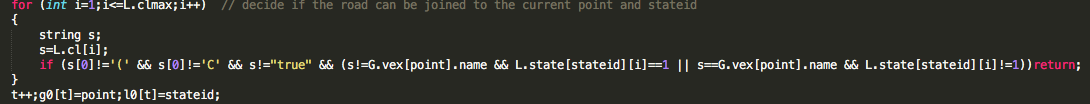
\includegraphics[scale=0.4]{2.png}
\end{figure}

接下来我们用$string$ $roadto[$ $][51]$数组记录下到达这个顶点的道路信息。

\begin{figure}[!htb]
\centering
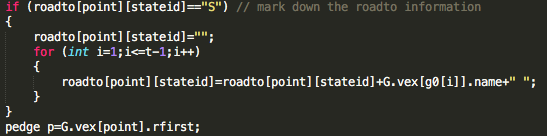
\includegraphics[scale=0.5]{3.png}
\end{figure}

然后进入深度优先搜索的过程,我们利用一个循环语句判断下一个位置能否到达。

\begin{figure}[!htb]
\centering
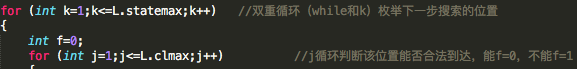
\includegraphics[scale=0.5]{4.png}
\end{figure}

接下来我们判断是否形成回路,并保存回路的信息。

\begin{figure}[!htb]
\centering
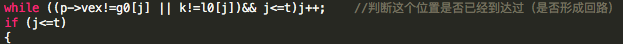
\includegraphics[scale=0.5]{5.png}
\end{figure}

\begin{figure}[!htb]
\centering
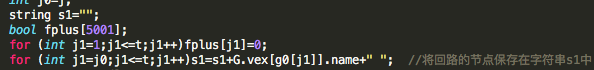
\includegraphics[scale=0.5]{6.png}
\end{figure}

我们对于新找到的回路,判断它是否满足了$final[10]$中存储的某个出现$U$“直到”算符的子串,如果有新满足的子串的话,我们记录下来,并且扩充之前得到的回路,使得整个回路满足更多这样的子串。

\begin{figure}[!htb]
\centering
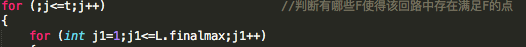
\includegraphics[scale=0.5]{7.png}
\end{figure}

\begin{figure}[!htb]
\centering
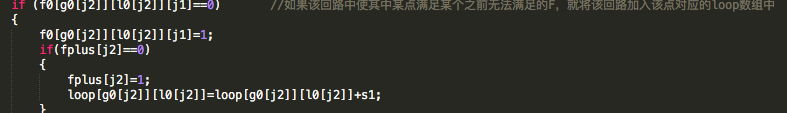
\includegraphics[scale=0.5]{8.png}
\end{figure}

最后我们如果没有形成回路,就继续递归探索,并最终回到之前状态进行回溯。

\begin{figure}[!htb]
\centering
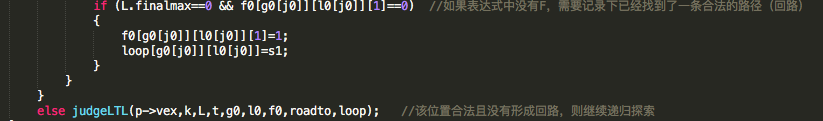
\includegraphics[scale=0.5]{9.png}
\end{figure}

\begin{figure}[!htb]
\centering
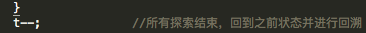
\includegraphics[scale=0.5]{10.png}
\end{figure}

\section{模型的评价与改进}


\subsection{模型的优点}
(1)处理$CTL$模型检验时,我们的算法在思想上和具体实现上都十分简单,程序的复杂度也很低,我们可以容易地处理大规模的模型检验运算。

(2)处理$LTL$模型检验时,我们的算法将反例化归到回路情况,能够在较短的时间内给出反例。

(3)我们将输入输出标准化,存储在文件里,判断具体的模型检验时就显得一目了然了。

\subsection{模型的缺点}
(1)在$LTL$模型检验中,我们的程序在时间复杂度和空间复杂度上都显得太过于复杂,深度搜索引入了近乎难以容忍的运算量,于是$LTL$的算法只能解决比$CTL$模型检验规模小的多的问题。

(2)程序的交互性做的不够好,不能达到一个较好的可视化界面的设计。

\subsection{模型的改进与推广方向}
(1)从处理$CTL$模型检验时候的逆推算法设计我们可以看出,这个算法不仅思想简明易懂,还具有很强的普适性,我们可以援引同样的算法来处理解决$CTL$*、$PCTL$、$TCTL$等模型检验的问题。例如本质上$TCTL$就是考虑到时间因素的$CTL$模型,逆推的过程中考虑时间元素即可,同样的$PCTL$中状态出现的概率也可以朴素的使用逆推来完成计算,并比较输出检验成果。至于$CTL$*,在本质上是$LTL$与$CTL$模型检验算法的整合,我们利用逆推算法来拆解$CTL$*逻辑公式,在必要的逆推步骤时利用$LTL$模型检验得到的结果。(当然特别的,在$CTL$*、$PCTL$、$TCTL$的问题中,自然在一般情况下也没有枚举反例的意义)

(2)在$LTL$模型检验中,我们可以引入更多的逻辑判断,来在第一阶段就筛选掉不合逻辑的状态转化(即我们减少新图$G_{1}$的顶点与边数,这样一来减少了深度优先算法搜索的规模,模型在时间复杂度层面上便能够进一步得到简化),只不过这些逻辑组的判断需要引入更多的数组,会增加空间复杂度。由此可见,我们的模型应该在时间与空间复杂度上追求一个平衡状态。

(3)最后,我们想探究是否能不借助状态转化的思想,构造新图$G_{1}$,来检验$LTL$模型。我们的算法中这样新图的构造使得程序的空间复杂度本身就显得极为庞大,深度搜索的时间复杂度更是达到了近乎难以接受的程度,如果能够类似于处理$CTL$模型的逆推方法,同时解决无穷逆推的问题,就能给出一个时间消耗上精简很多的的算法。

\section{模型的完成心得}
这次的模型建立总的来说还是花去了我们不少功夫。本以为朴素的算法,在实现过程中却发现一些技术上难以克服的问题,在一筹莫展之际,我们参照提供的幻灯片讲稿与参考书找到了解决$LTL$模型检验的算法,最终解决了这个庞大的工程。另外,我们也自己设计了一些简单的逻辑筛查函数,大幅减少了程序的时间复杂度。值得一提的是在编写代码的过程中,考虑到代码的简洁性,我们设置了多个具有明显实际意义的函数,并尽量精简程序,最终得到一个较为紧凑的结构。

\newpage
\begin{center}
  \bf{\LARGE 附录}
\end{center}
\appendix
\renewcommand{\appendixname}{Appendix~\Alph{section}}
\section{使用的软件}
\subsection{编程软件}
$Cpp$:$Dev-C++$   \&  $Sublime$  $Text$                  

\subsection{报告及幻灯片软件}
\LaTeX:\TeX Shop

\section{代码及文件}
本模型的代码主要建立在一个主程序的基础上,另外还有一个输入文件,用具体的算例来检验这个模型检验的算法是否符合要求,在输出文件中我们列出了模型检验得到的结果。此外,我们压缩包里还附有上机报告以及幻灯片展示的$PDF$文件。

\section{小组成员的具体工作}
我们在完成模型设计的过程中,进行了如下的分工合作:

(1)算法设计:韩啸、王逸轩

(2)程序代码实现:韩啸

(3)上机报告及程序注释:王逸轩、韩啸

(4)幻灯片展示:王逸轩

	\end{document}
